% Preámbulo
\documentclass[12pt,a4paper]{article} % Documento del tipo artículo
\usepackage[utf8]{inputenc} % utf8
\usepackage{amsmath} % Matemática
\usepackage[T1]{fontenc} % Fuentes
\usepackage{amsfonts} % Matemática
\usepackage{amssymb} % Matemática
\usepackage[spanish,es-tabla]{babel} % Idioma
\usepackage{makeidx} % 
\usepackage{hyperref} % Vínculos
\usepackage{graphicx} % Gráficas
%\usepackage{subfig} % Subfiguras ---------- Revisar el error que genera
\usepackage{cite} % Citas
\usepackage{lmodern} %
\usepackage{listings} %
\usepackage{xcolor} % Color
\usepackage{float} % Figuras
\usepackage{xfrac} %
\usepackage{fix-cm} %
\usepackage{titlesec} %
\usepackage{setspace} %
\usepackage{fancyhdr} %
\usepackage{lipsum} % Textos
\usepackage{appendix}
\usepackage{caption}
\usepackage{subcaption}
\usepackage{tikz}
\usepackage{caption}
\captionsetup[table]{
   name = Tabla,
   labelsep = newline,
   justification = raggedright,
   singlelinecheck = false,
   labelfont = bf
}
\renewcommand{\thesection}{\Roman{section}}
\renewcommand{\thesubsection}{\arabic{section}.\arabic{subsection}}
\AtBeginDocument{\renewcommand{\contentsname}{ÍNDICE}}
\onehalfspace
\titleformat{\section}
{\bfseries\large}
{\large\thesection. }
{1pt}
{}

% Personalización del documento
\fancyhead[L]{}
\fancyhead[C]{}
\fancyhead[R]{}
\fancyfoot[L]{}
\fancyfoot[C]{}
\fancyfoot[R]{\thepage}
\renewcommand{\headrulewidth}{0pt}
\renewcommand{\footrulewidth}{0pt}

\graphicspath{{imagenes/}}
\usepackage[margin = 2.54cm]{geometry} % Geometría
\setlength{\parindent}{0cm} % Sangría


% Entorno del documento
\begin{document}

\pagestyle{empty} %

% Carátula
\begin{titlepage}
	\begin{center}
		{\textbf{UNIVERSIDAD}}\\
		{\textbf{FACULTAD}}\\
		{\textbf{ESCUELA PROFESIONAL}}\\
		\vspace{2cm}
			\begin{figure}[h]
				\centering
				
\includegraphics[height=7cm]{EXAMEN_FINAL/Imagenes/logo-unsch.png}
			\end{figure}
		\vspace{2mm}
				\begin{center}
					{\textbf{TÍTULO DE LA TESIS}}
				\end{center}
	  \vspace{1cm}
			{\bf Tesis}\\
		\vspace{2mm}
			{\textit{Bachiller o título profesional}}\\
    \vspace{1cm}
			{\bf Autor}\\
		\vspace{2mm}
			{Nombre completo del autor}\\
		\vspace{4mm}
    	{\bf Asesor}\\
		\vspace{2mm}
			{Nombre completo del asesor}\\
	  \vspace{16mm}
			{CIUDAD, AÑO}\\
	  \vspace{2mm}
			{PAÍS}
	\end{center}
\end{titlepage}


\newpage % Nueva página
\setcounter{page}{1}
\pagestyle{fancy} % Estilo de página

\tableofcontents % Tabla de contenidos
\listoffigures  % Índice de figuras
\listoftables % Índice de tablas


\newpage

% Introducción
\section*{INTRODUCCIÓN}
\addcontentsline{toc}{section}{INTRODUCCIÓN}
    \lipsum[1-3]


% Planteamiento del problema
\newpage
\section{PLANTEAMIENTO DEL PROBLEMA}
    %% Enunciado del problema
    \subsection{Enunciado del problema}
    	\lipsum[4]

    %% Formulación del problema
    \subsection{Formulación del problema}
    	\lipsum[5]
        %%% Problema general
        \subsubsection{Problema general}
        	\lipsum[6]
        %%% Problemas específicos
        \subsubsection{Problemas específicos}
        	Un texto es una composición de signos codificados en un sistema
					de escritura que forma una unidad de sentido. También es una composición de caracteres imprimibles generados por un algoritmo de cifrado que, aunque no tienen sentido para cualquier persona, sí puede ser descifrado por su destinatario original.


% Objetivos
\newpage
\section{OBJETIVOS}
    %% Objetivo general
    \subsection{Objetivo general}
    	\lipsum[8]
    %% Objetivos específicos
    \subsection{Objetivos específicos}
    	\lipsum[9]

			\lipsum[10]

			\lipsum[11]


% Justificación
\newpage
\section{\hspace{0.5mm} JUSTIFICACIÓN}
	\lipsum[10]

	\lipsum[11]

	\lipsum[12]

	\lipsum[13]

	\lipsum[14]


% Marco teórico
\newpage
\section{\hspace{0.5mm} MARCO TEÓRICO}
    %% Marco histórico
    \subsection{Marco histórico}
    	\lipsum[11]

    %% Sistema teórico
    \subsection{Sistema teórico}
    	\lipsum[12]

    %% Marco conceptual
    \subsection{Marco conceptual}
    	\lipsum[13]

    %% Marco referencial
    \subsection{Marco referencial}
    	\lipsum[14]


% Hipótesis
\newpage
\section{HIPÓTESIS}
    %% Hipótesis general
    \subsection{Hipótesis general}
    	\lipsum[15]

    %% Hipótesis específicos
    \subsection{Hipótesis específicos}
    	\lipsum[16]

			\lipsum[17]

			\lipsum[18]


% Variables e indicadores
\newpage
\section{VARIABLES E INDICADORES}
    \lipsum[17]
		% Tabla
		\begin{table}[h]
        \raggedright
        \caption{Variables e indicadores}
          \begin{tabular}{|c|c|}
             \hline
             Variables & Indicadores \\
             \hline
             Variable 1 & Indicador 1\\
             Variable 2 & Indicador 2\\
             Variable 3 & Indicador 3\\
             Variable 4 & Indicador 4\\
            \hline
           \end{tabular}
         \vspace{2mm}
        \caption*{\it Nota: Elaboración propia.}
        \label{tab: Variables e indicadores}
    \end{table}
		\lipsum[1]

		\begin{table}[h]
        \raggedright
        \caption{Variables e indicadores}
          \begin{tabular}{|c|c|}
             \hline
             Variables & Indicadores \\
             \hline
             Variable 1 & Indicador 1\\
             Variable 2 & Indicador 2\\
             Variable 3 & Indicador 3\\
             Variable 4 & Indicador 4\\
            \hline
           \end{tabular}
         \vspace{2mm}
        \caption*{\it Nota: Elaboración propia.}
        \label{tab: Variables e indicadores}
    \end{table}

% Metodología
\newpage
\section{\hspace{1mm} METODOLOGÍA}
		\lipsum[1]
			\begin{equation}
				Y_{i} = \beta_{1} + \beta_{2}X_{2i} + \cdots + \beta_{k}X_{ki} + \mu_{i}
			\end{equation}
		\lipsum[1]
			\begin{figure}[h]
				\centering
				\caption{Motivos por las cuales dejaron de operar}
				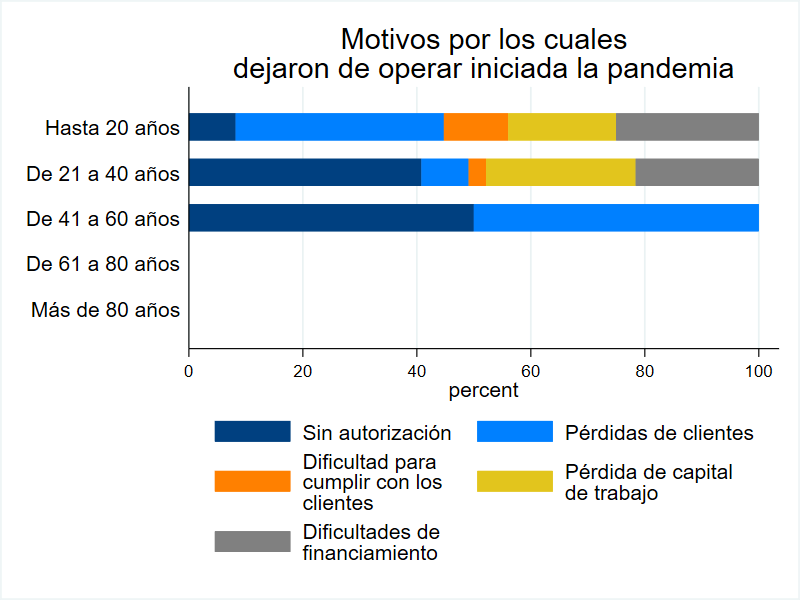
\includegraphics[height=7cm]{EXAMEN_FINAL/Imagenes/Graph2.png}
				\label{fig: Motivos por las cuales dejaron de operar}
			\end{figure}
		\lipsum[1]
		\vspace{0.7cm}\\
		\textcolor{red!75}{Equivalence between DC and SE}. Under usual
		regularity conditions (convexity and Inada conditions), and given
		$b^{i}(s^{0}) = \text{for all} \quad i \in I$, the allocations of the Debreu
		competitive equilibrium and the allocations of the sequential equilibrium
		are equivalent. Moreover, the spence of wages and interest rates are the same, and

		\begin{equation}
				Q(s^{t+1}|s^{t}) = \frac{q(s^{t+1})}{q(s^{t})} =
				\beta \frac{U_{c}^{i}(s^{t+1})}{U_{c}^{i}(s^{t})} \frac{\pi(s^{t+1})}{\pi(s^{t})}
		\end{equation}

		for all $ t, s^{t}$, and $s^{t+1}|s^{t}$.

    %% Tipo y nivel de investigación
    \subsection{Tipo y nivel de investigación}
			\lipsum[1]
			\begin{figure}[h]
				\centering
				\caption{Distribución de las empresas}
				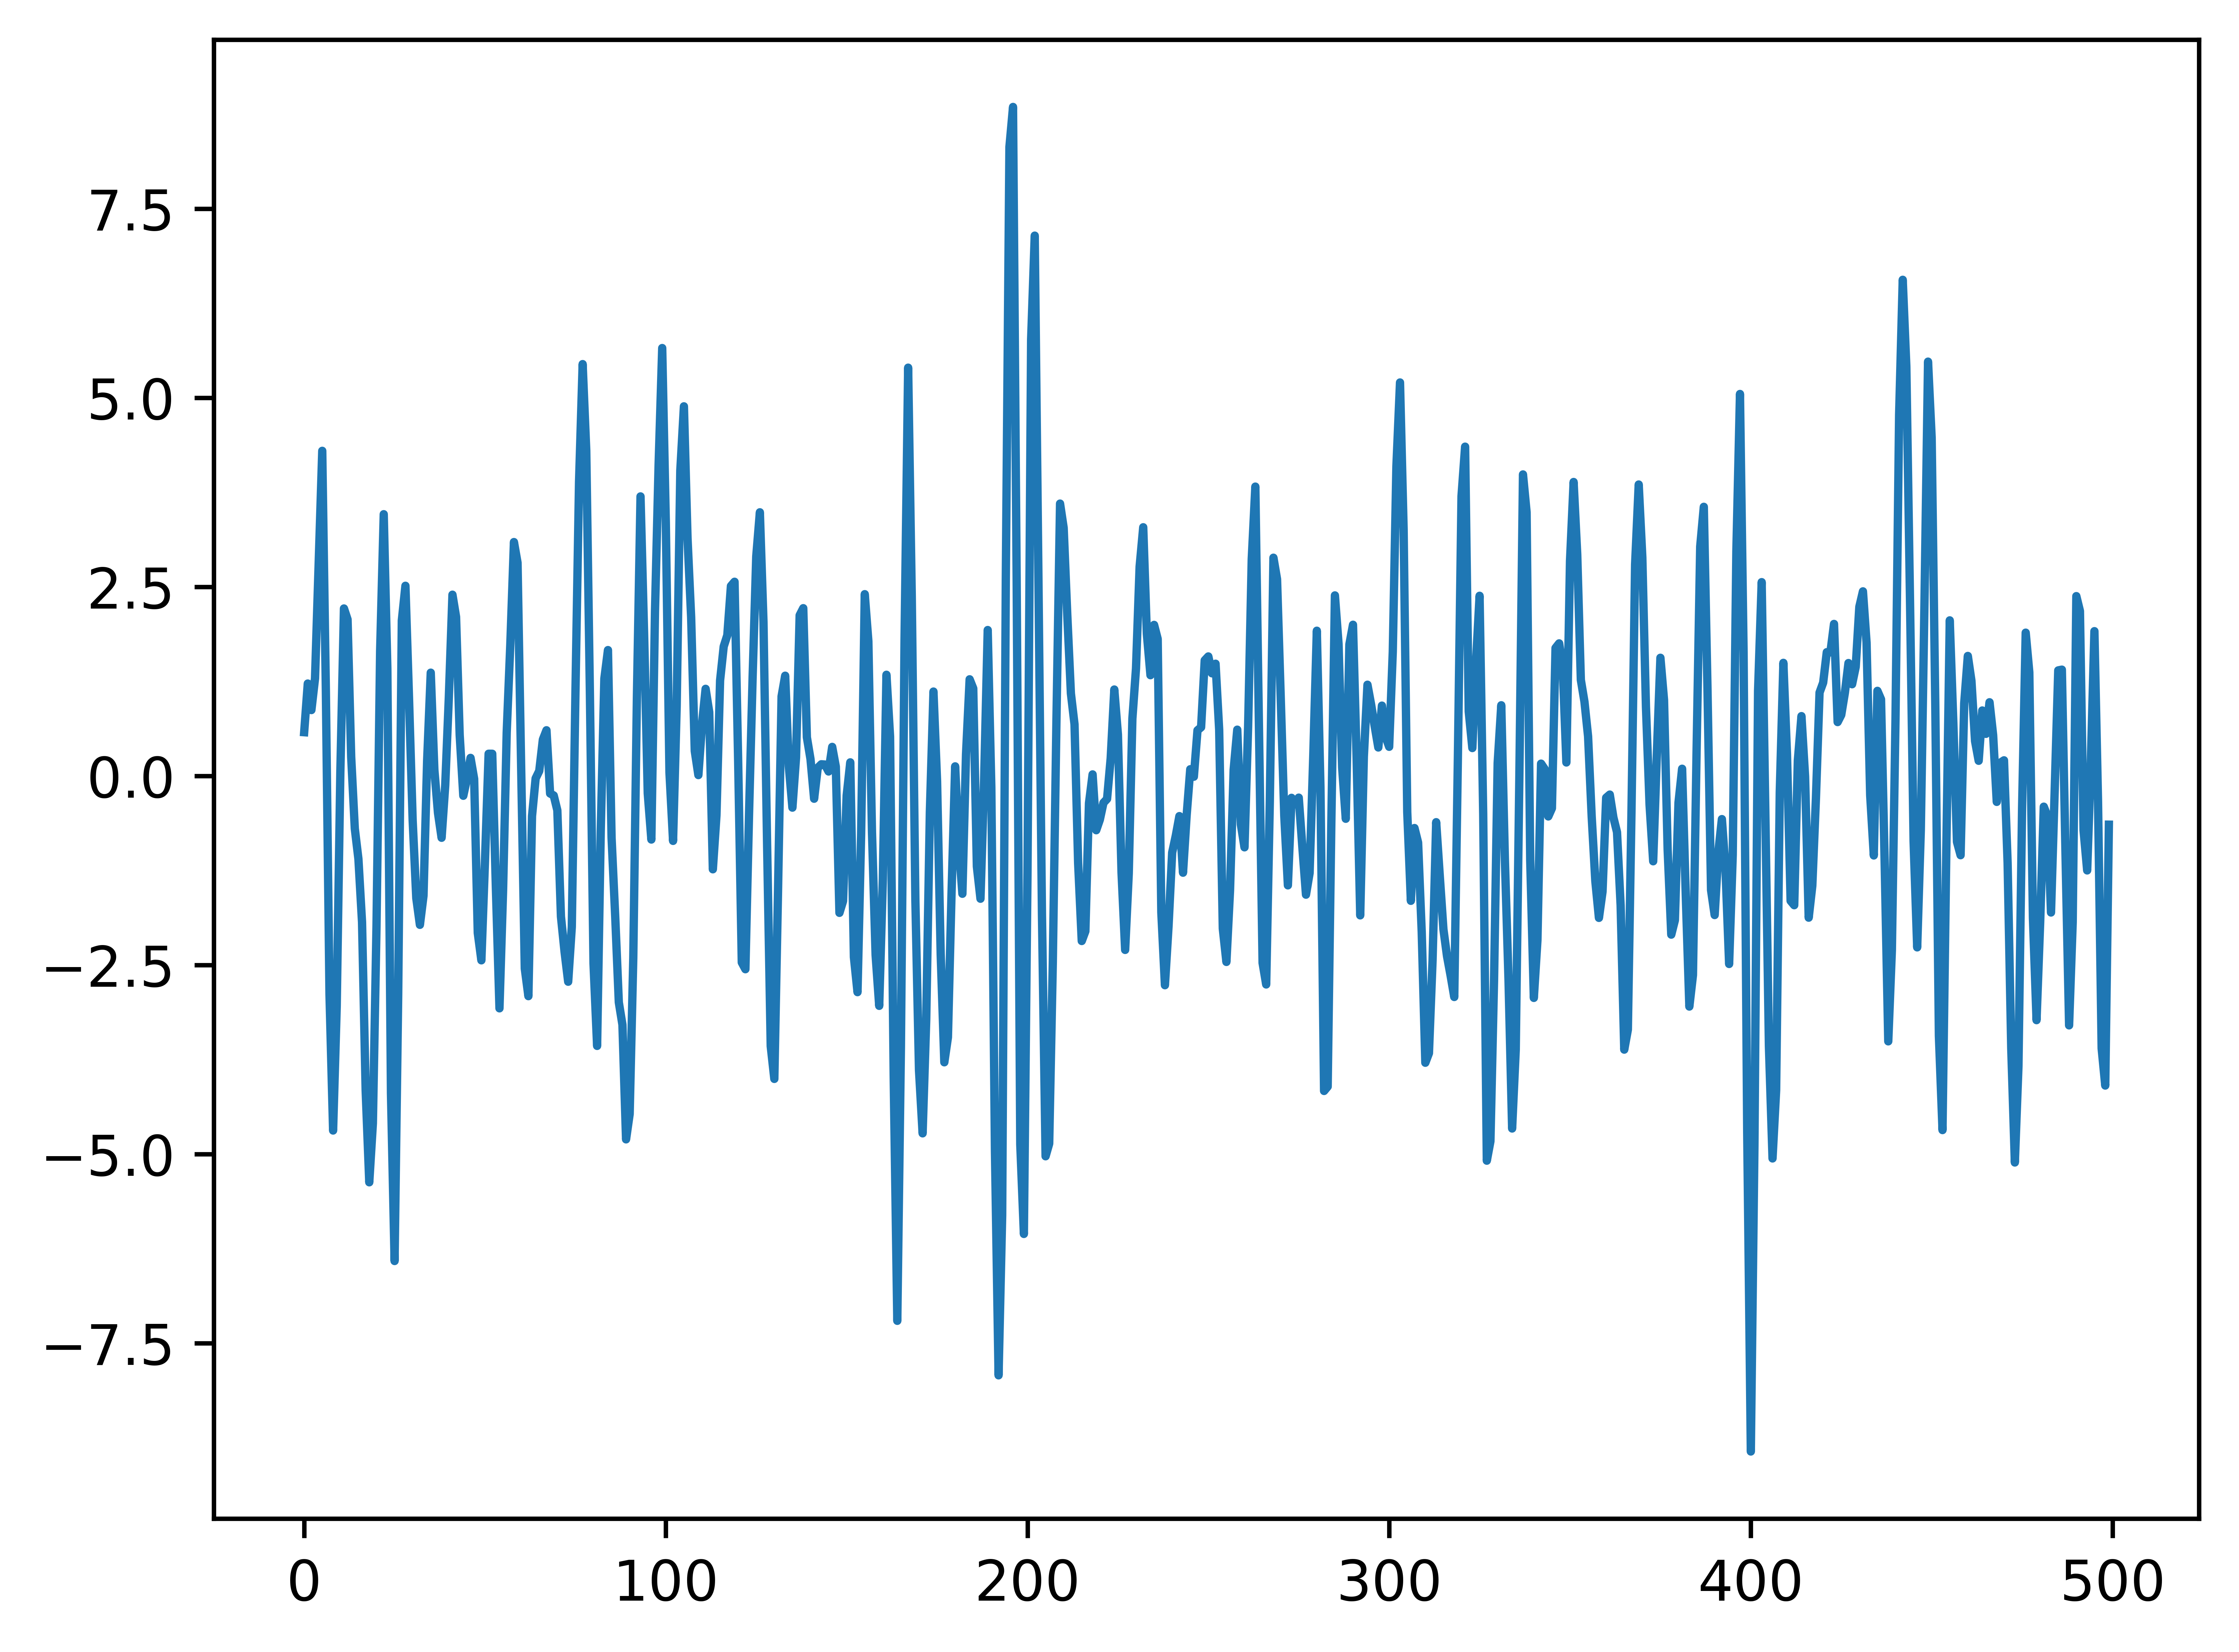
\includegraphics[height=7cm]{EXAMEN_FINAL/Imagenes/Graph1.png}
				\label{fig: Distribución de las empresas}
			\end{figure}

    %% Población y muestra
    \subsection{Población y muestra}
			\lipsum[1]
			\begin{figure}[ht]
      	\centering
        \begin{subfigure}[b]{0.3\textwidth}
        	\centering
          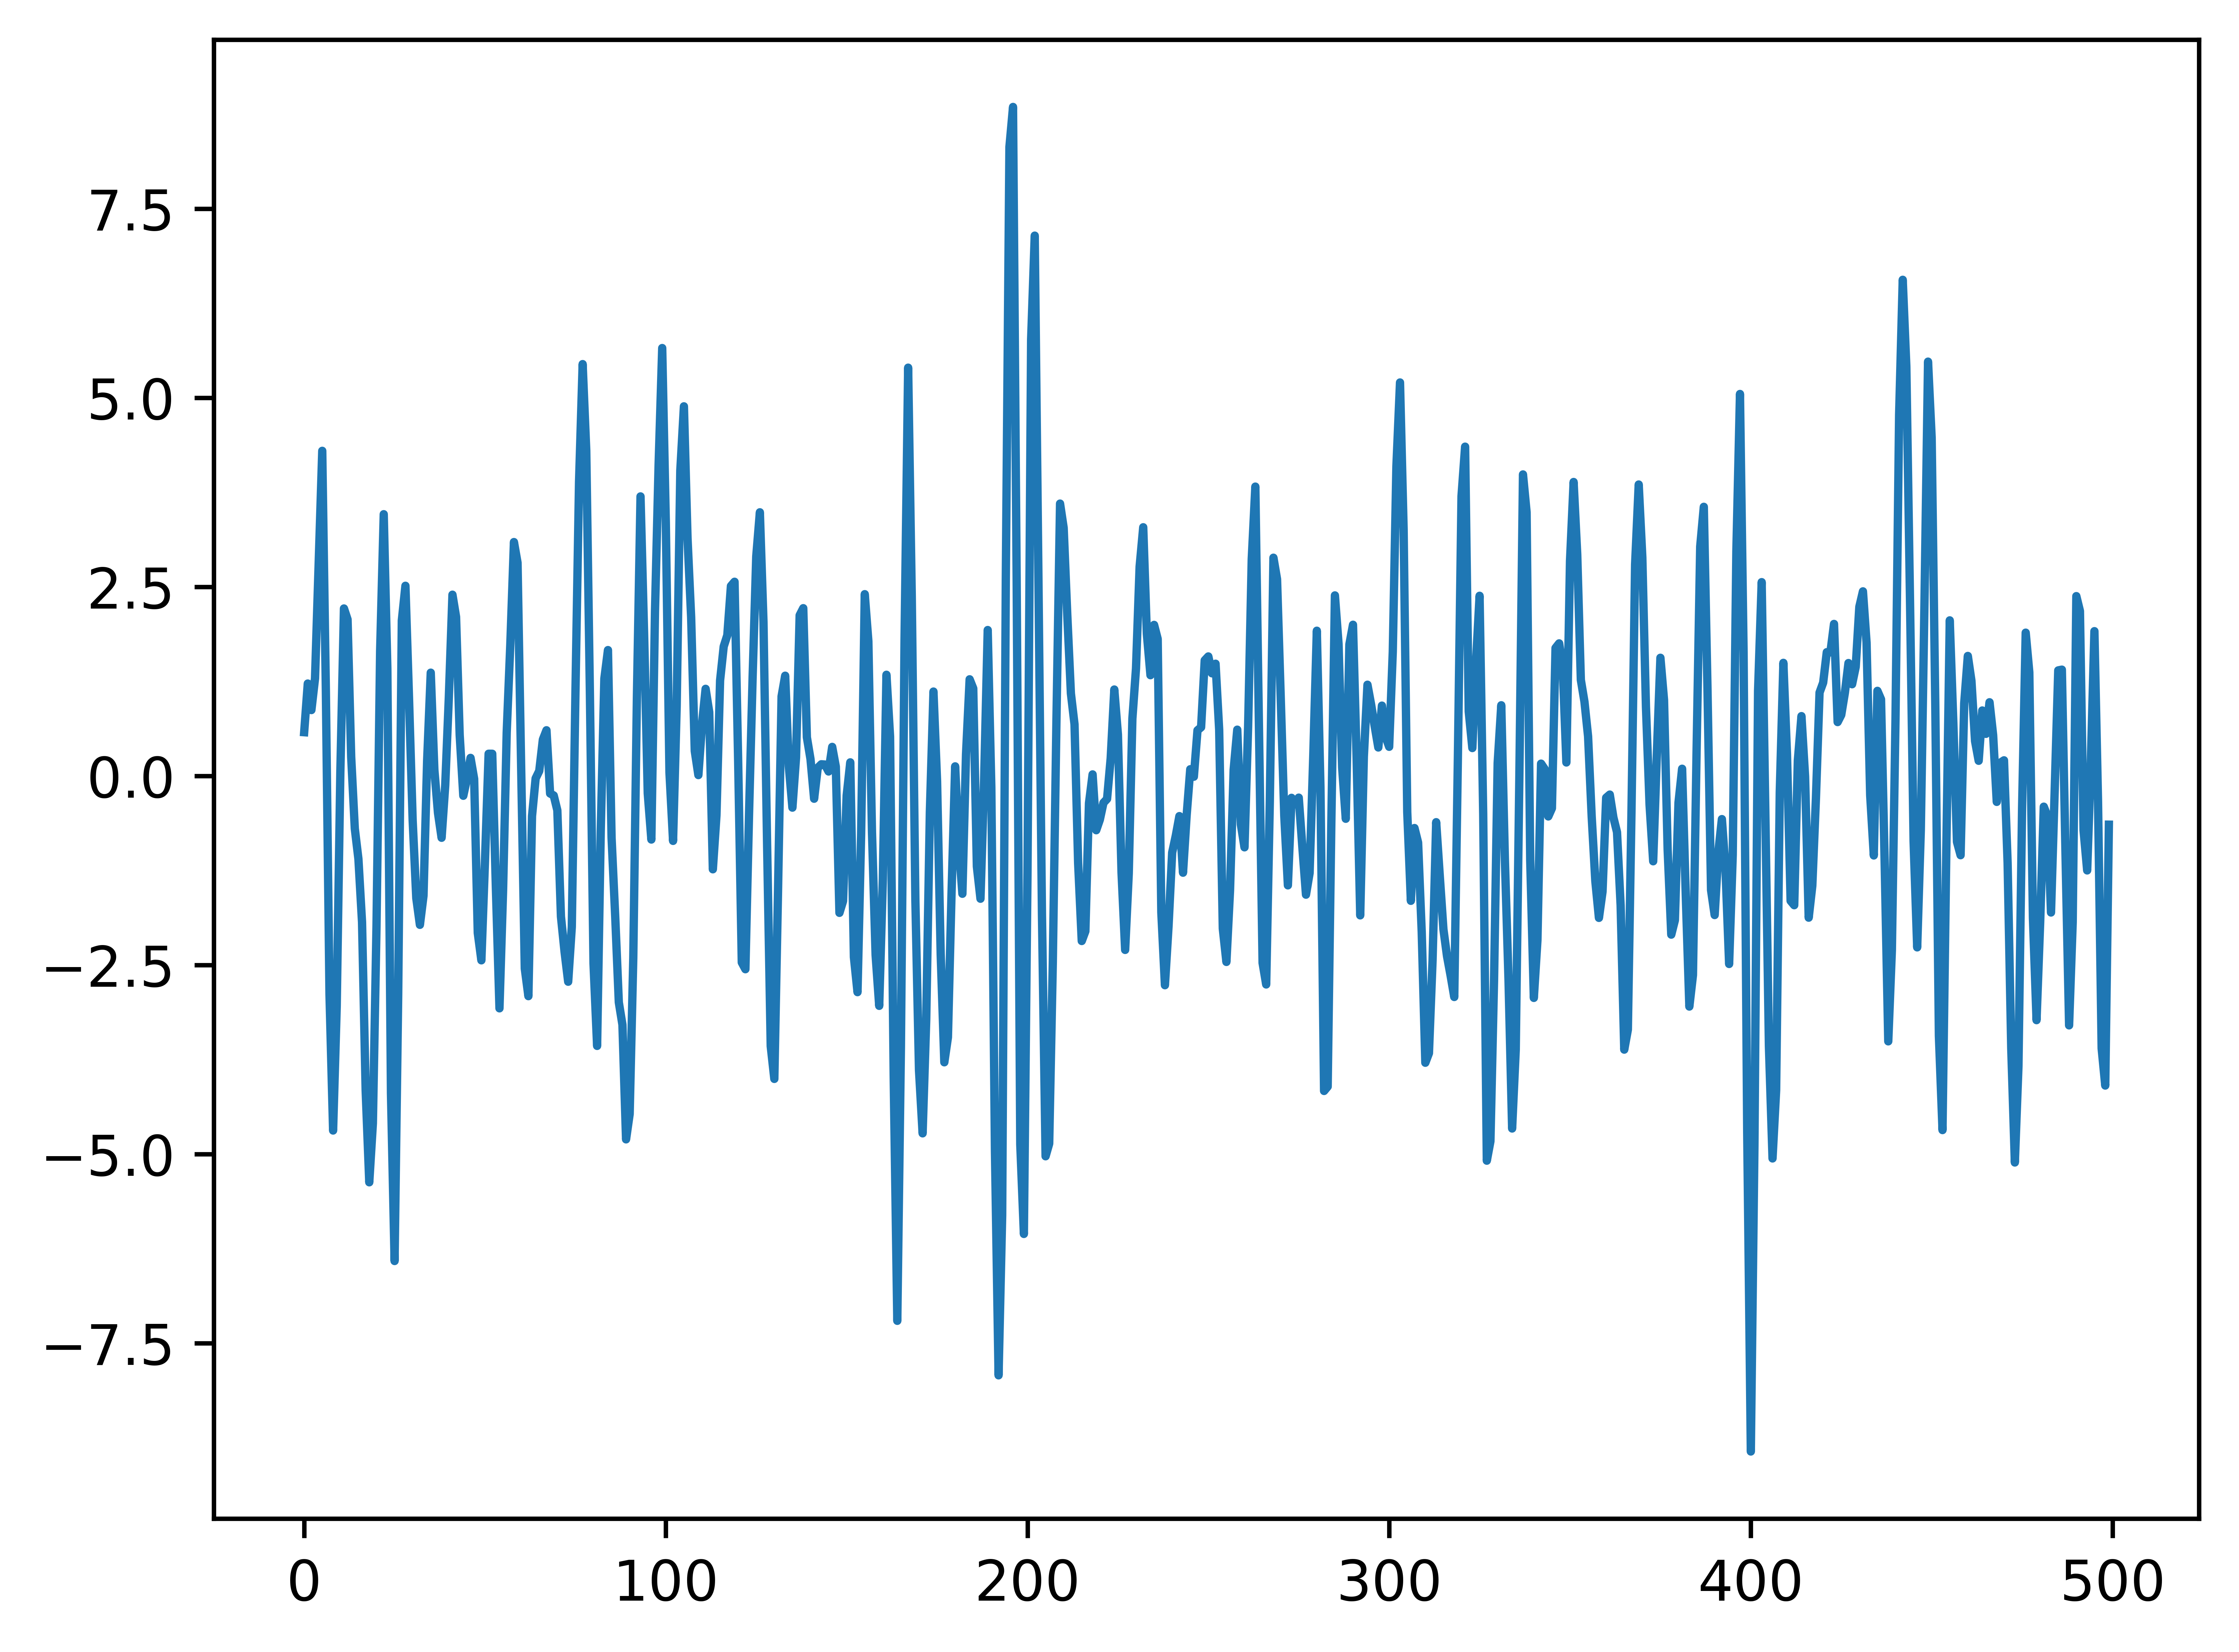
\includegraphics[width=\textwidth]{EXAMEN_FINAL/Imagenes/Graph1.png}
          \caption{Distribución}
          \label{fig: Distribución}
        \end{subfigure}
        \hfill
        \begin{subfigure}[b]{0.3\textwidth}
        	\centering
          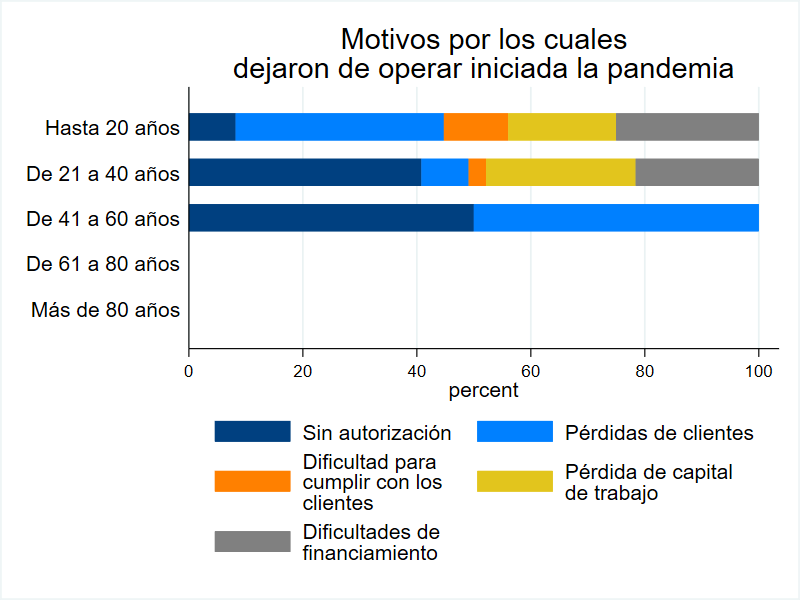
\includegraphics[width=\textwidth]{EXAMEN_FINAL/Imagenes/Graph2.png}
          \caption{Motivo}
          \label{fig: Motivo}
        \end{subfigure}
        \hfill
        \begin{subfigure}[b]{0.3\textwidth}
        	\centering
          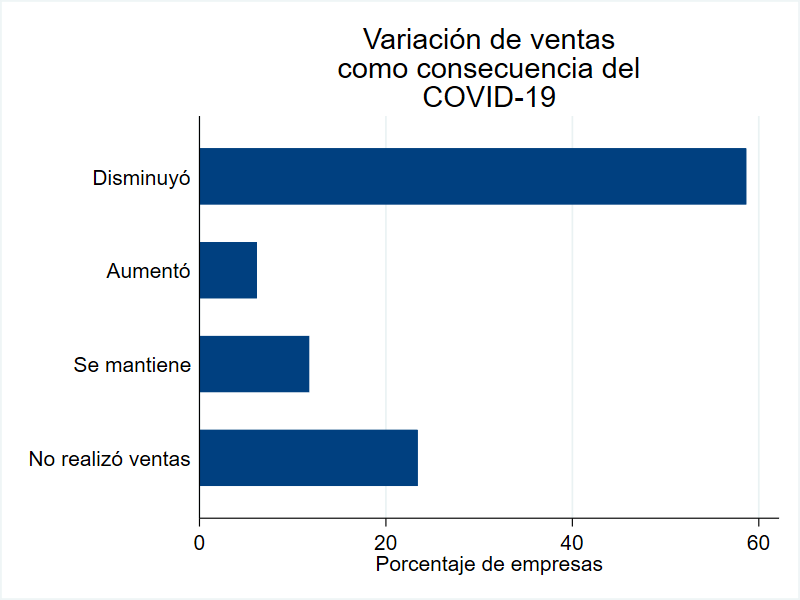
\includegraphics[width=\textwidth]{EXAMEN_FINAL/Imagenes/Graph3.png}
          \caption{Ventas}
          \label{fig: Ventas}
        \end{subfigure}
        	\caption{Situación de las empresas en la pandemia}
        	\label{fig: Situación de las empresas en la pandemia}
    \end{figure}

    %% Fuentes de información
    \subsection{Fuentes de información}
			\lipsum[1]
			\begin{figure}[h]
				\centering
				\caption{Variación de ventas}
				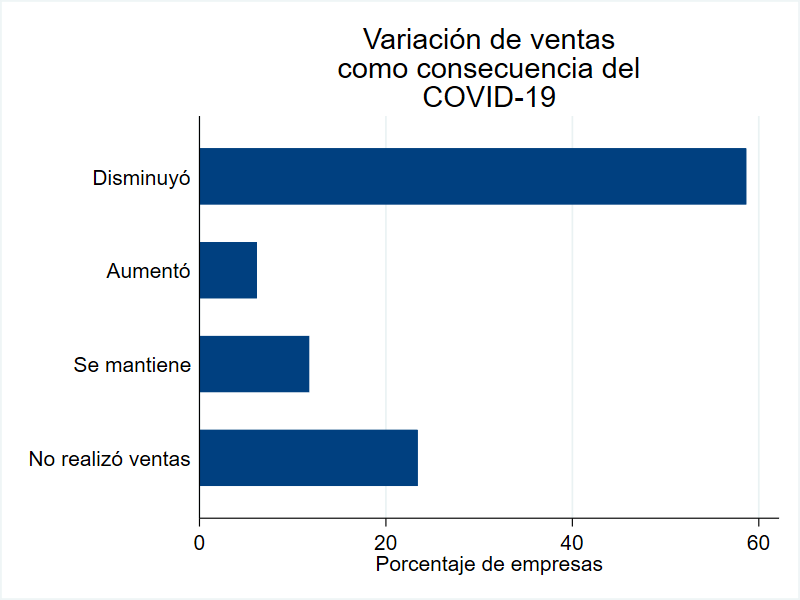
\includegraphics[height=7cm]{EXAMEN_FINAL/Imagenes/Graph3.png}
				\label{fig: Variación de ventas}
			\end{figure}


    %% Diseño de investigación
    \subsection{Diseño de investigación}
			\lipsum[1]
			\begin{figure}[h]
				\centering
				\caption{Preguntas}
				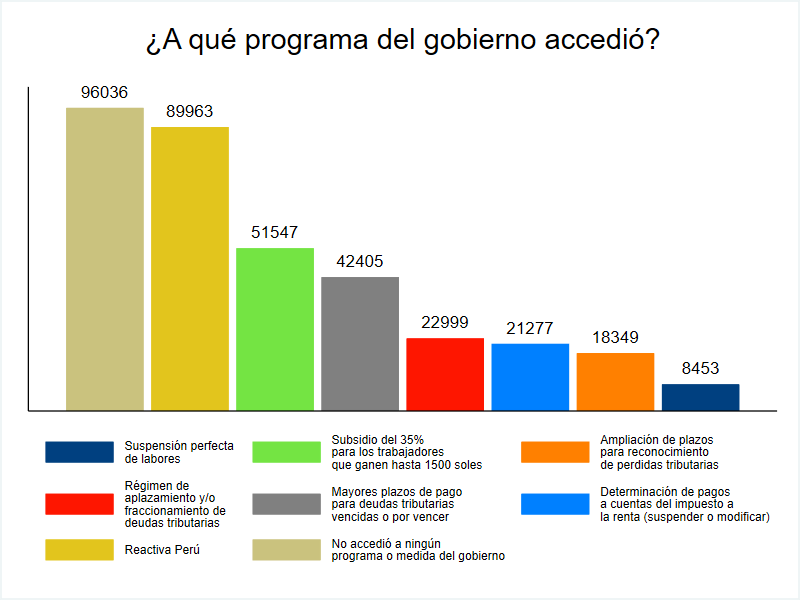
\includegraphics[height=7cm]{EXAMEN_FINAL/Imagenes/Graph4.png}
				\label{fig: Preguntas}
			\end{figure}

    %% Técnicas e instrumentos
    \subsection{Técnicas e instrumentos}
			\lipsum[1]
			\begin{figure}[H]
        \centering
        \begin{tikzpicture}
            \draw[blue, dashed, very thick, fill = lightgray] (1,1) circle[radius = 2];
            \draw[fill = black] (1,1) circle[radius = 0.05];
            \node[below right] at (1,1) {$(1,1)$};
            \draw[green] (-3,-4) rectangle (1,-2);
            \draw[<-] (1,1) -- (1,3) -- (1,3) -- (1,3);
		  \draw[darkgray, dashed] (-6, 1) -- (6, 1);
            \draw[darkgray, dashed] (-6, 2) -- (6, 2);
            \draw[darkgray, dashed] (-6, 3) -- (6, 3);
            \draw[darkgray, dashed] (-6, 4) -- (6, 4);
            \draw[darkgray, dashed] (-6, 5) -- (6, 5);
            \draw[darkgray, dashed] (1, -5) -- (1, 5);
            \draw[darkgray, dashed] (2, -5) -- (2, 5);
            \draw[darkgray, dashed] (3, -5) -- (3, 5);
            \draw[darkgray, dashed] (4, -5) -- (4, 5);
            \draw[darkgray, dashed] (5, -5) -- (5, 5);
            \draw[darkgray, dashed] (-1, -5) -- (-1, 5);
            \draw[darkgray, dashed] (-2, -5) -- (-2, 5);
            \draw[darkgray, dashed] (-3, -5) -- (-3, 5);
            \draw[darkgray, dashed] (-4, -5) -- (-4, 5);
            \draw[darkgray, dashed] (-5, -5) -- (-5, 5);
            \draw[<-, red] (6,0) -- (-6,0);
            \draw[<-, red] (0,6) -- (0,-6);
        \end{tikzpicture}
        \caption{Mi imagen usando Tikz}
        \label{fig: Tikz}
    \end{figure}

		\lipsum[1]

% Referencias bibliográficas
\newpage
\section{\hspace{2.5mm} REFERENCIAS BIBLIOGRÁFICAS}
    %% Estilo APA
    	\bibliographystyle{apa}
        	\begin{thebibliography}{4}
            	\bibitem{C1} Cita sdjadajsdhasdashdashdggasdasgda
							\bibitem{C2} Csdasd
							\bibitem{C3} asasa
							\bibitem{C4} asdada
							\bibitem{C5} ajhda
        	\end{thebibliography}



% Anexos
\newpage
\section{\hspace{0.5mm} ANEXOS}
    %% Anexo 1
    \subsection{ANEXO 1: Matriz de consistencia}
			\begin{table}[H]
				\centering
				\caption{Matriz de consistencia}
					\begin{tabular}{p{5cm}p{5cm}p{5cm}}
						\hline
						Problema & Objetivo & Hipótesis\\
						\hline
						\lipsum[1] & \lipsum[1] & \lipsum[1]\\
						\hline
					\end{tabular}
				\label{tab: Matriz de consistencia}
			\end{table}

    %% Anexo 2
    \subsection{ANEXO 2: Resultados }
			\begin{table}[H]
				\centering
				\caption{Tabla de resultados}
					\begin{tabular}{p{5cm}p{5cm}p{5cm}}
						\hline
						Resultado 1 & Resultado 2 & Resultado 3\\
						\hline
						\lipsum[1] & \lipsum[1] & \lipsum[1]\\
						\hline
					\end{tabular}
				\label{tab: Resultados}
			\end{table}

			%% Anexo 3
	    \subsection{ANEXO 3: Datos }
				\begin{table}[H]
					\centering
					\caption{Datos}
						\begin{tabular}{p{5cm}p{5cm}p{5cm}}
							\hline
							Variable 1 & Variable 2 & Varaible 3\\
							\hline
							\lipsum[1] & \lipsum[1] & \lipsum[1]\\
							\hline
						\end{tabular}
					\label{tab: Datos}
				\end{table}



\end{document}
